\chapter*{Introducción}
En el año 1758, Euler publica un artículo que cubre diversas propiedades de los poliedros. El principal resultado de su artículo es la celebrada fórmula de Euler para poliedros convexos,
\[V-A+C=2\]
La demostración de este resultado se basa en el hecho de que los poliedros convexos son homeomorfos a un sólido común, la bola cerrada. Si consideramos un poliedro irregular que sea homeomorfo a la esfera, este resultado sigue siendo válido.

Sin embargo, podemos encontrar poliedros que no verifiquen esta fórmula eliminando la condición de convexidad. Un ejemplo de poliedro que no verifica esta expresión es el tetrahemihexaedro, con 6 vértices, 12 aristas y 7 caras. Si computamos su valor $V-A+C$, obtenemos
\[6-12+7=1\]

\begin{marginfigure}
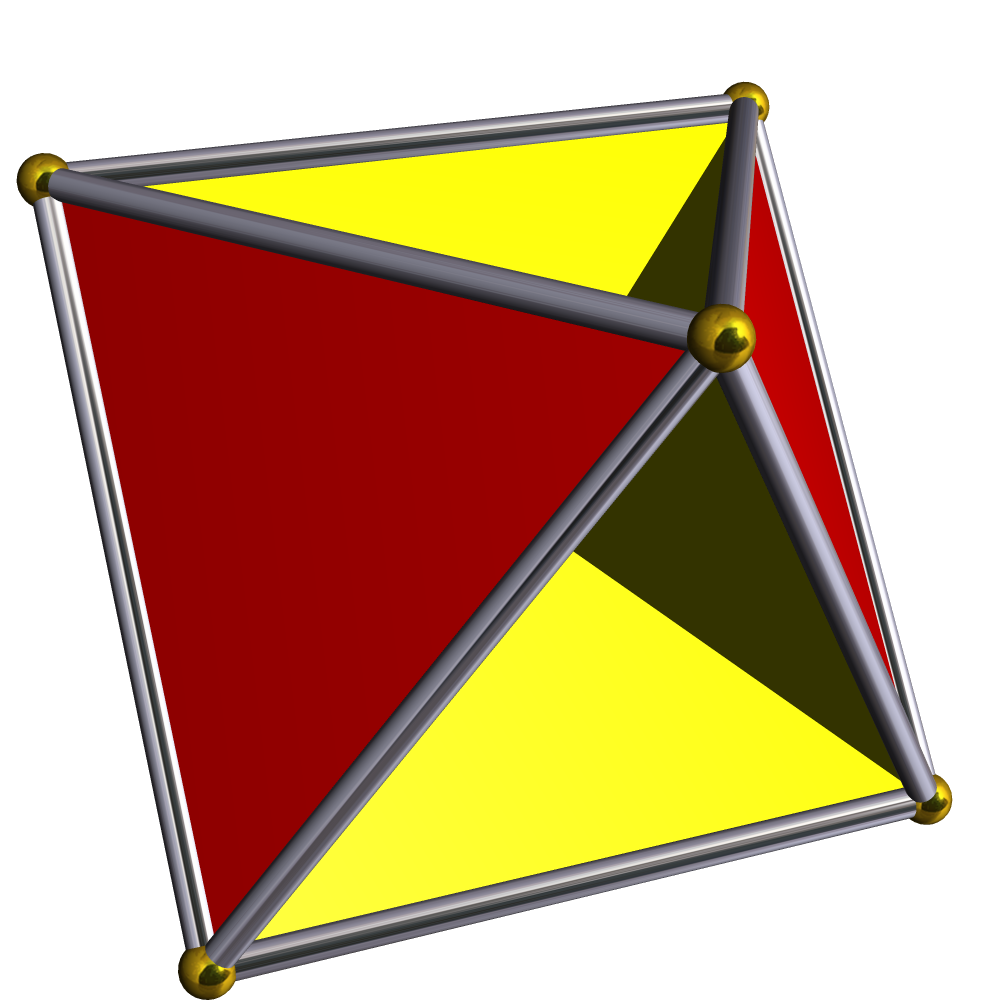
\includegraphics{Figures/Tetrahemihexahedron.png}
%https://en.wikipedia.org/wiki/Euler_characteristic#/media/File:Tetrahemihexahedron.png
\caption[Tetrahemihexaedro]{Tetrahemihexaedro regular. Algunas de sus caras se intersecan entre sí, haciendo que su topología sea diferente a la de la bola cerrada.}
\end{marginfigure}

El valor $V-A+C$ de un poliedro regular se denomina \emph{característica de Euler} del poliedro.

Un espacio topológico $X \subset \mb{R}^n$ 2AN y Hausdorff es una superficie si, dado $p \in X$, existe un entorno abierto $U \subset X$ de $p$ homeomorfo a una bola de $\mb{R}^2$. Desde un punto de vista geométrico, podemos decir que los puntos de $X$ perciben el mundo en dos dimensiones, al igual que los personajes de la novela \emph{Planilandia}. Algunas superficies pueden ser representadas utilizando poliedros regulares, que podemos clasificar en función de su característica de Euler. Cuando una superficie sea homeomorfa a algún poliedro regular, diremos que es poliédrica.

A partir de un espacio topológico, podemos generar una familia de grupos abelianos llamados \emph{grupos de homología}. Los grupos de homología nos permiten utilizar técnicas de álgebra conmutativa para conocer algunas de las propiedades topológicas de un espacio, permitiendo probar resultados que están fuera del alcance de la topología conjuntista. En particular, veremos una demostración del teorema del punto fijo de Brouwer, que establece la existencia de puntos fijos para cualquier aplicación continua entre conjuntos convexos.

El objetivo de este texto es introducir al lector en la teoría de homología singular, y está dirigido principalmente a estudiantes de la \emph{Universitat de València}. Como consecuencia, el lector se asume familiarizado con el contenido cubierto por las asignaturas de Estructuras algebraicas y Topología de segundo curso.
